%%%%%%%%%%%%%%%%%%%%%%%%%%%%%%%%%%%%%%%%%%%%%%%%%%%%%%%%%%%%%%%%%%%%%%%%%%%%%%%%
%2345678901234567890123456789012345678901234567890123456789012345678901234567890
%        1         2         3         4         5         6         7         8

\documentclass[letterpaper, 10 pt, conference]{ieeeconf}  % Comment this line out
                                                          % if you need a4paper
%\documentclass[a4paper, 10pt, conference]{ieeeconf}      % Use this line for a4
                                                          % paper

\IEEEoverridecommandlockouts                              % This command is only
                                                          % needed if you want to
                                                          % use the \thanks command
\overrideIEEEmargins
% See the \addtolength command later in the file to balance the column lengths
% on the last page of the document

\usepackage{cite}
\usepackage[pdftex]{graphicx}
\graphicspath{{../pdf/}{../jpeg/}}
\DeclareGraphicsExtensions{.pdf,.jpeg,.png,.eps}
\usepackage{epstopdf}
\usepackage[cmex10]{amsmath}
\usepackage{subfig}
\usepackage{dblfloatfix}
\usepackage{color}
\usepackage{amsmath,multicol}

\usepackage{algorithm}
\usepackage{algorithmic}

% The following packages can be found on http:\\www.ctan.org
%\usepackage{graphics} % for pdf, bitmapped graphics files
%\usepackage{epsfig} % for postscript graphics files
%\usepackage{mathptmx} % assumes new font selection scheme installed
%\usepackage{times} % assumes new font selection scheme installed
%\usepackage{amsmath} % assumes amsmath package installed
%\usepackage{amssymb}  % assumes amsmath package installed

%
% paper title
% can use linebreaks \\ within to get better formatting as desired
\title{\LARGE \bf
Stabilizing a Quadruped robot locomotion\\ using a 2 Degree of Freedome Tail}


%\author{ \parbox{3 in}{\centering Huibert Kwakernaak*
%         \thanks{*Use the $\backslash$thanks command to put information here}\\
%         Faculty of Electrical Engineering, Mathematics and Computer Science\\
%         University of Twente\\
%         7500 AE Enschede, The Netherlands\\
%         {\tt\small h.kwakernaak@autsubmit.com}}
%         \hspace*{ 0.5 in}
%         \parbox{3 in}{ \centering Pradeep Misra**
%         \thanks{**The footnote marks may be inserted manually}\\
%        Department of Electrical Engineering \\
%         Wright State University\\
%         Dayton, OH 45435, USA\\
%         {\tt\small pmisra@cs.wright.edu}}
%}

%\author{Huibert Kwakernaak$^{1}$ and Pradeep Misra$^{2}$% <-this % stops a space
%\thanks{*This work was not supported by any organization}% <-this % stops a space
%\thanks{$^{1}$H. Kwakernaak is with Faculty of Electrical Engineering, Mathematics and Computer Science,
%        University of Twente, 7500 AE Enschede, The Netherlands
%        {\tt\small h.kwakernaak at papercept.net}}%
%\thanks{$^{2}$P. Misra is with the Department of Electrical Engineering, Wright State University,
%        Dayton, OH 45435, USA
%        {\tt\small p.misra at ieee.org}}%
%}

% author names and affiliations
% use a multiple column layout for up to three different
% affiliations

\author{Alan Mutka, Matko Orsag, and Zdenko Kovacic% <-this % stops a space
\thanks{The work presented in this paper was carried out within the project “Integrated Control of Robotic Systems in Complex Environments“ that is supported by a grant from the Croatian Ministry of Science, Education and Sports.}% <-this % stops a space
\thanks{A. Mutka, M. Orsag and Z. Kovacic are with the Laboratory for Robotics and Intelligent Control Systems, Universirty of Zagreb, Croatia, {\tt\small\{amutka, morsag, zkovacic\}{@}fer.hr}}
}

\begin{document}

\maketitle
\thispagestyle{empty}
\pagestyle{empty}

%%%%%%%%%%%%%%%%%%%%%%%%%%%%%%%%%%%%%%%
% Abstract
\begin{abstract}
%\boldmath
This paper presents the use of a tail for quadruped robot locomotion in order to apply additional forces/torques to stabilize the motion during flight phases in which the robot has no contact with the ground. The paper presents a Denavit-Hartenberg parameterization based kinematics of a two degree of freedom tail combined with a Newton-Euler based dynamic model. Impedance based leg control simplifies the leg motion so that it can be modeled as a dampened spring system. Finally, a recursive algorithm that moves the tail in order to balance the robot is proposed. A realistic model of the robot is built in Open Dynamic Engine environment and is used to conduct a series of tests proving the effectiveness of the proposed algorithm.
%Compared to autonomous ground vehicles, UAVs (unmanned aerial vehicles) have significant mobility advantages and the potential to operate in otherwise unreachable locations. Micro UAVs still suffer from one major drawback: they do not have the necessary payload capabilities to support high performance arms. This paper, however, investigates the key challenges in controlling a mobile manipulating UAV using a commercially available aircraft and a light-weight prototype 3-arm manipulator. Because of the overall instability of rotorcraft, we use a motion capture system to build an efficient autopilot. Our results indicate that we can accurately model and control our prototype system given significant disturbances when both moving the manipulators and interacting with the ground.
\end{abstract}

% IEEEtran.cls defaults to using nonbold math in the Abstract.
% This preserves the distinction between vectors and scalars. However,
% if the conference you are submitting to favors bold math in the abstract,
% then you can use LaTeX's standard command \boldmath at the very start
% of the abstract to achieve this. Many IEEE journals/conferences frown on
% math in the abstract anyway.

% no keywords


%%%%%%%%%%%%%%%%%%%%%%%%%%%%%%%%%%%%%%%
% Introduction
\section{Introduction}\label{sec:introduction}
% no \IEEEPARstart

Animals utilize tails in a variety of ways: to propel themselves through water; to help improve locomotion and balance; and some even use their tails for hanging on branches or for grasping trees. Balance control while running and hopping, or while gliding and climbing are just few examples of how a tail can help animals to realize robust locomotion \cite{Thomas:Nature2012}. The use of a tail for dynamic stabilization has been reported in the case of dinosaurs, lizards, cats, primates and even humans \cite{ostrom1969osteology,PijnappelsSringer,Walker199841,JusufiIOP2010}. One of the challenges in the design of biologically inspired robot systems is studying phenomena in natural systems and extracting basic knowledge for building similar technical systems. This does not mean only mimicking the nature, but also searching for innovative solutions. One such challenge is to add a tail mechanism to a walking robot so that it improves robot locomotion in a similar way as an animal's tail would do. 
 
A tail can balance the robot's body in both static and dynamic sense. The main technique of using a tail as a dynamic stabilizer for quadruped robot locomotion is to apply additional forces/torques on its body. Uniroo \cite{zeglin1991uniroo} is one of the first robots which uses a single degree of freedom active tail to maintain constant body pitch with the purpose of emulating a hopping kangaroo. Another active tail stabilization case presented in \cite{conf/iros/Chang-SiuLTF11} uses a tail on a wheeled car as a means for robust maneuvering on uneven terrain and stable pitch control by applying the principle of conservation of the momentum. The MIT Cheetah robot \cite{DBLP:conf/iros/BriggsLHK12} uses a tail to improve robot's running capabilities and perform runs up to 30 mph. Additionally, the authors analyze several other artificial mechanisms which can be used for exerting non-contact forces/torques like a reaction wheel, reaction mass, thrusters etc. In \cite{PullinICRA12}, Pullin et all compared the use of a tail to classical differential drive steering for different surface conditions on a crawling mobile robot OctoRoACH. They showed how a tail could be used when rapid turning or evasive maneuvers are required under low friction surface conditions. Learning from aerial robots, one can apply the techniques used in \cite{Korpela2013ICRA,Orsag2012JINT} to model the dynamics of inertial appendages and the impact they have on the underlying robot body. This paper however, wishes to address an alternative use for a tail, its static balancing capabilities. A tail is envisioned here as a counterweight capable of shifting its center of mass so as to balance effectively the robot body.
 
\begin{figure}
                \centering
                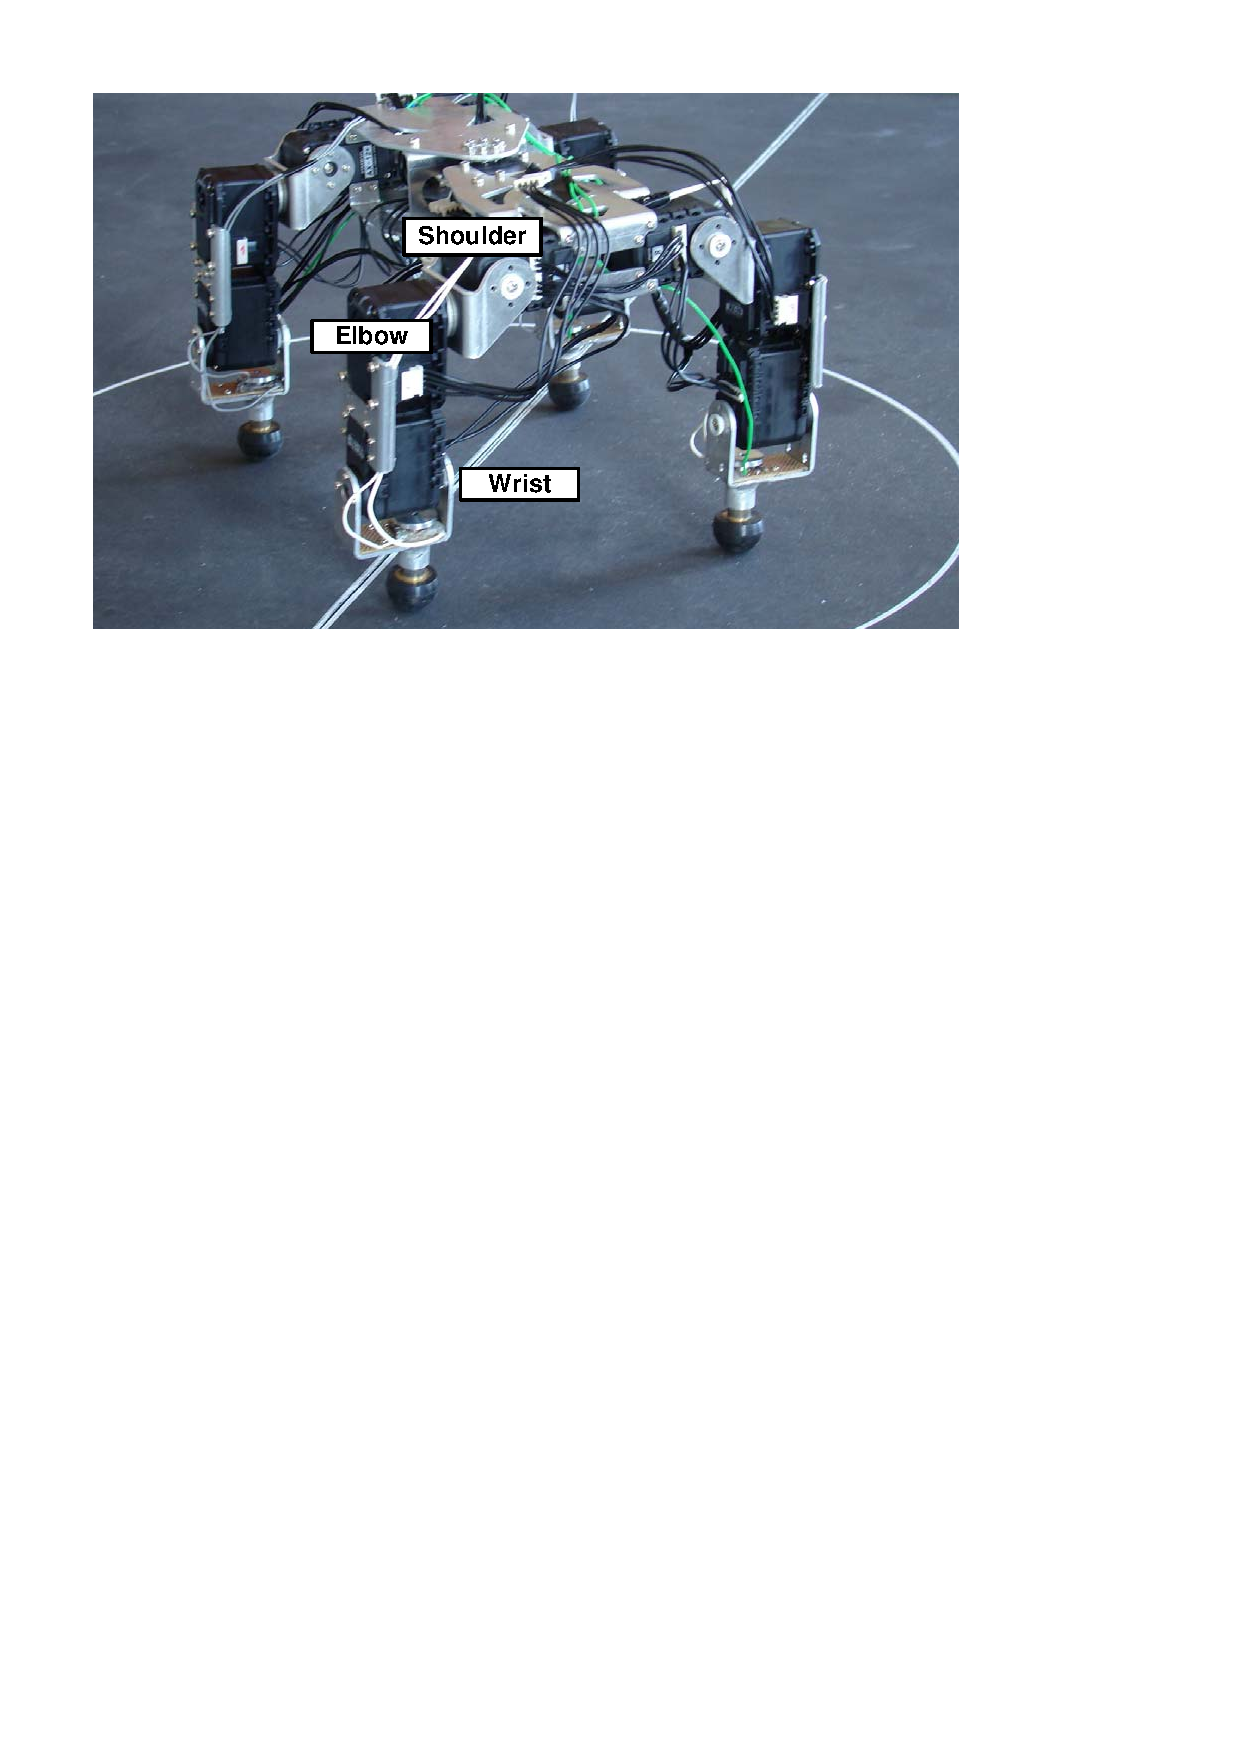
\includegraphics[width=75mm]{./pictures/Dynarobin_introduction_image.pdf}
                \caption{A quadruped robot Dynarobin \cite{DBLP:conf/IEEEcca/MutkaPRK12}}
                \label{fig:Dynarobin}
\end{figure}
 
Inspired by the agility of human and animal locomotion, over the last few decades the number of research groups presented numerous robot leg designs, and the associated modeling and control \cite{CambridgeJournals:1345088}. The predominant method for the modeling of quadruped locomotion gaits like walking, running, trotting, and bouncing is a spring-mass model\cite{Blickhan01}. This paper postulates that a single leg, hopping locomotion can also be described with a spring-mass model. In order to obtain a compliant robot leg behavior, impedance control is used to emulate a virtual spring-mass system \cite{Havoutis01}. By attaching four legs to one central body complex dynamic problems arise. In order to provide a stable quadruped hopping sequence a lot of parameters need to be observed: mass distribution, active and passive leg stiffness, ground stiffness, etc. This paper investigates how to improve locomotion stability of a dynamical system composed of four spring-masses by using a tail-like inertial appendage.
 
In Section \ref{sec:MathModel} a mathematical model of a quadruped robot Dynarobin (Fig. \ref{fig:Dynarobin}) together with a kinematic and a dynamic model of the tail is introduced. A single leg dynamics is modeled to mimic the behavior of an active spring-mass system. Building upon the results from Section \ref{sec:MathModel}, a recursive balancing algorithm is introduced in Section \ref{sec:Algorithm}. The algorithm is tested in the simulation environment which is described in Section \ref{sec:simulation}, along with the simulation results.




% Some research uses advanced variable stiffnes leg design %\cite{Hurst_2004_4785}\cite{Galloway}\cite{Jun:2009:DSV:1703775.1704089} which allows robot to run over a large variety %of terrains while adjusting their leg stiffness. All this research suggests that quadrupedal robot can be dynamically 5modeled as mass supported on four spring legs as shown in fig. 




%%%%%%%%%%%%%%%%%%%%%%%%%%%%%%%%%%%%%%%

%%%%%%%%%%%%%%%%%%%%%%%%%%%%%%%%%%%%%%%
% Dynarobin,Single leg model 
%
%\section{Dynarobin leg model}

%This paper goal is to improove locomotion stability on quadrupedal robot Dynarobin, depicted in Fig. \ref{fig:Dynarobin}. 
The robot has four identical legs ($l\in \left \{ 1,2,3,4 \right \}$), each combining three rotational joints: hip, knee, and ankle, respectively. Fig. \ref{fig:DynarobinLEG} depicts one such leg, with each joint marked with a red circle and an additional mechanical spring end-effector. In order to mimic the spring-mass system, each joint controller implements impedance control \cite{citeulike:2203614}. The actual implementation goes beyond the scope of this paper and will not be further discussed. Together with adequate joint trajectory planning and inverse kinematics the legs can be tuned to mimic the behavior of an active spring-mass system \cite{conf/iros/ParkP12}\cite{6171868}, so that when the legs are in the contact with the ground, side forces and thrust forces are produced.

Besides the kinematic chain performing as an active spring, each leg contains an additional mechanical spring that changes the stiffness of the contact with the surface. Combining these mechanical springs together with leg's compliant dynamics enables us to model each leg of the robot as a single, active spring. The simplified quadruped's leg model is shown in Fig. \ref{fig:DynarobinLEG}. It consists of three masses connected by virtual active and passive springs. The passive spring has initial fixed length $L_{pl}=L_{p0}$ and parameters $K_{pl}$ and $C_{pl}$.  The actuated spring has variable parameters $K_{al}$ and $C_{al}$ and actuation is provided by changing the initial length $L_{al}=L_{a0}$ by $\Delta L$.
\begin{figure}[t!]
	\centering
	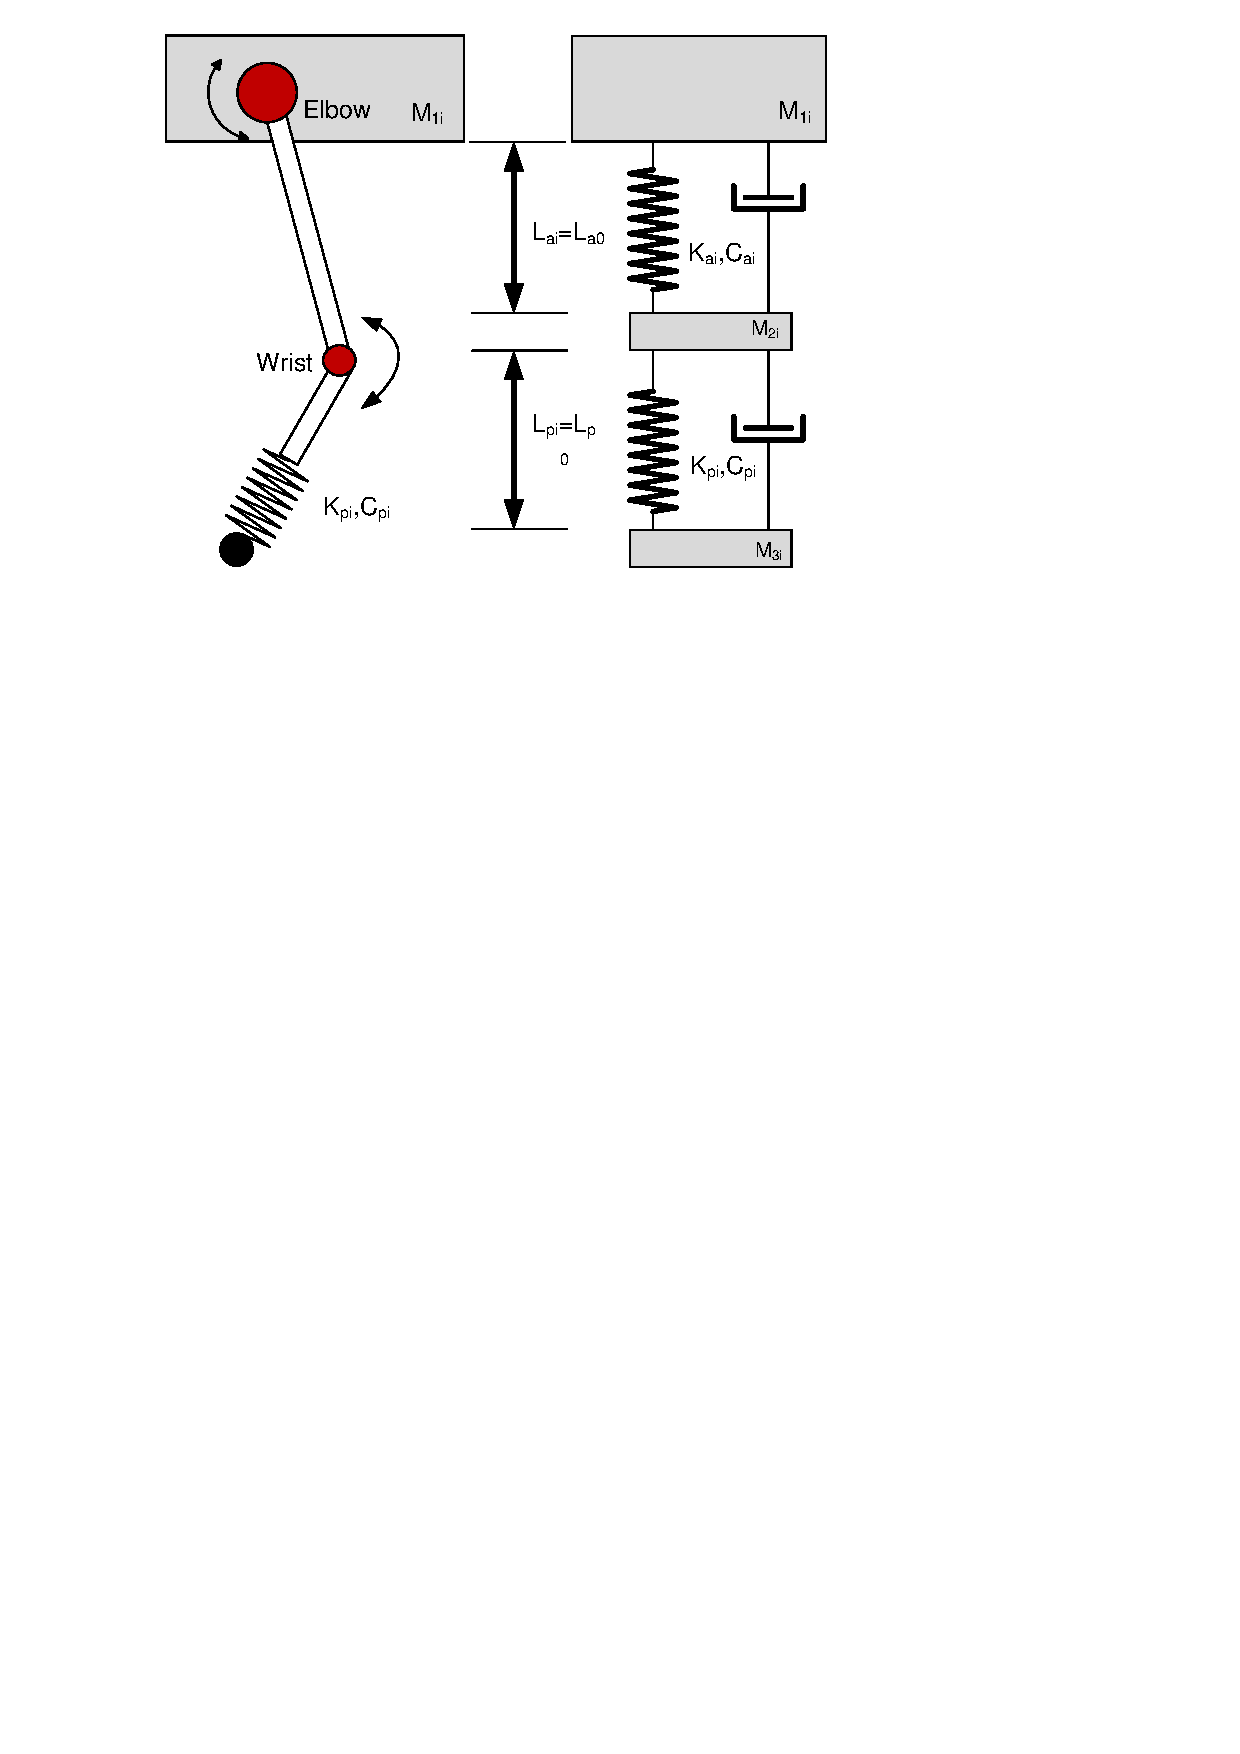
\includegraphics[width=80mm]{./pictures/Dynarobin_leg.pdf}
	\caption{Double spring-mass model of the leg}
	\label{fig:DynarobinLEG}
\end{figure}


%%%%%%%%%%%%%%%%%%%%%%%%%%%%%%%%%%%%%%%

%%%%%%%%%%%%%%%%%%%%%%%%%%%%%%%%%%%%%%%
% Mathematical model
\section{Mathematical model}\label{sec:MathModel}
A simplified model of a quadruped robot, depicted in Fig. \ref{fig:rmoment}, has three distinctive parts: the main body, the tail and four legs. Let the frame $L$ be defined with its origin $\vec{O}$ and the respective coordinate system, then the following key frames should be observed: $L_w$ - world frame, $L_c$ - geometrical center of construction frame; $L_B$ - main body's center of mass frame; $L_T$ - tail's center of mass frame; and $L_{pi}$ - $i$-th leg point of contact frame. The proposed mathematical model is derived under the assumption of a stable locomotion maneuver which includes vertical (jumping) and horizontal movement of the robot. For such a maneuver, the legs need to develop periodic horizontal and vertical forces denoted as side force $\vec{\textbf{S}}_{pi}$ and thrust force $\vec{\textbf{T}}_{pi}$ respectively. In order to achieve these forces, an adequate leg joint trajectory needs to be planned. Trajectory planning for the leg joints goes beyond the scope of this paper. 

\begin{figure}
	\centering
	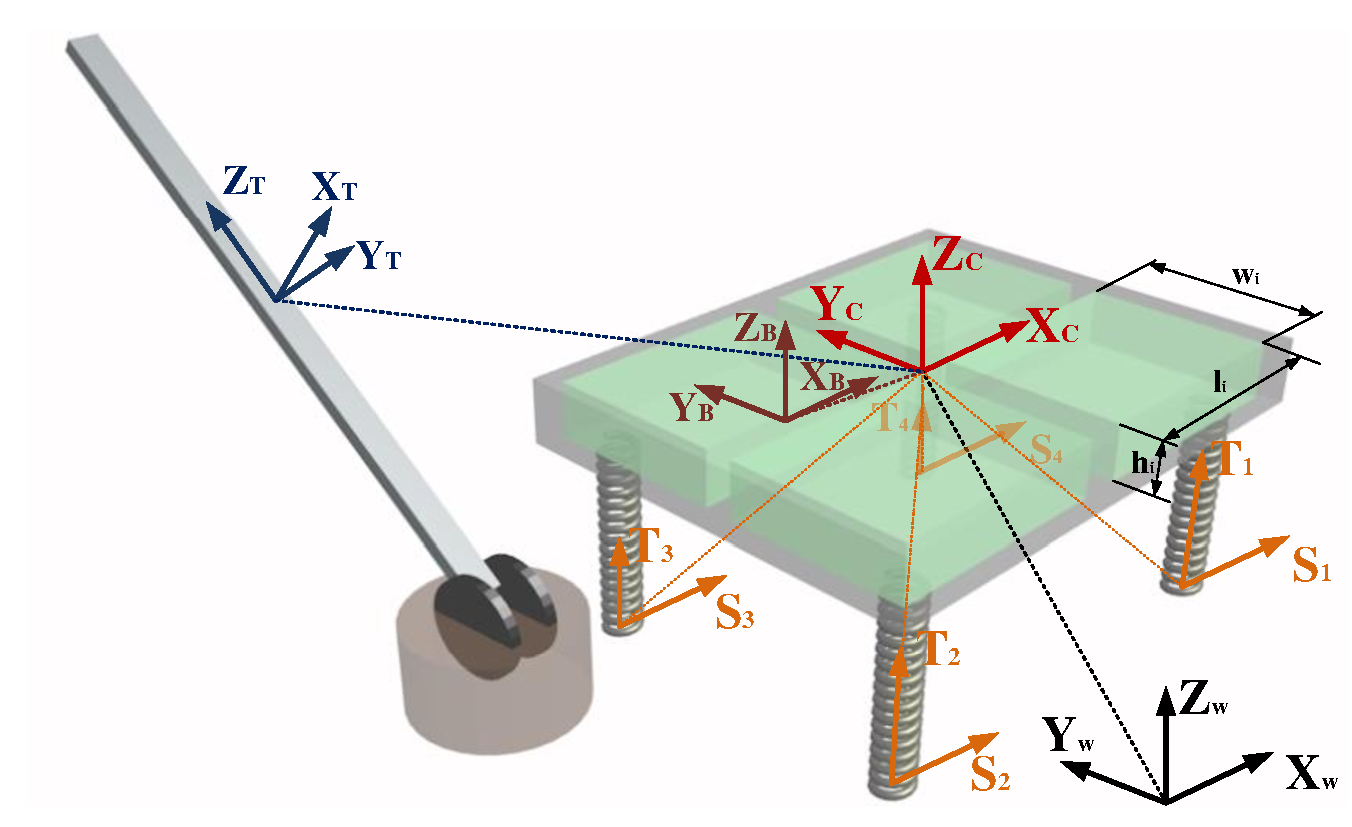
\includegraphics[width=85mm]{./pictures/RobinMoment.pdf}
	\caption{Symplified quadruped body dynamics}
	\label{fig:rmoment}
\end{figure}

\subsection{Main body dynamics}
In order to simplify the complexity of the analysis, quadruped's main body is modeled as a system of four, equally displaced cuboids, as shown in Fig \ref{fig:rmoment}. Ideally, when the robots's body is fully symmetric, all four parts have the same mass. Since, in most situations, this is not the case, each body element has its own mass $m_i$, with its own centroid $\vec{\textbf{cm}}_i$. Each centroid $\vec{\textbf{cm}}_i$ is then placed at $\vec{\textbf{r}}_i$ distance from the body geometric center, the $L_c$ coordinate system. The overall main body center of mass is then easily calculated with:
 
\begin{equation}\label{eq:CMrobot}
\vec{\textbf{r}_{CM}}=\frac{\sum_{i=1}^{4}m_i\vec{\textbf{r}}_i}{\sum_{i=1}^{4}m_i}
\end{equation}
Vector $\vec{\textbf{r}_{CM}}$ points from the center of construction frame $L_C$ to the center of mass frame $L_B$, quantifying the displacement of the center of mass from the construction center of the robot. All vectors are written with respect to the $L_c$ frame. Next important dynamic parameter is the tensor of inertia. Having four prismatic bodies as the basis for the robot model, tensor of inertia can easily be derived using the Parallel axis theorem:

\begin{equation}
\footnotesize
\textbf{J}_R=\sum_{i=1}^{4}\left \{\textbf{J}_{c_i}+m_i\begin{bmatrix}
{_yr_i}^2+{_zr_i}^2 & {_xr_i}\cdot {_yr_i} & {_xr_i}\cdot {_zr_i} \\ 
-{_xr_i}\cdot {_yr_i} & {_xr_i}^2+{_zr_i}^2 & {_yr_i}\cdot {_zr_i}\\ 
-{_xr_i}\cdot {_zr_i} & {_yr_i}\cdot {_zr_i} & {_yr_i}^2+{_xr_i}^2
\end{bmatrix} \right \}
\normalsize
\end{equation}

where, $_xr_i, _yr_i, _zr_i$ represent the $x,y,z$ projection of $\vec{\textbf{r}}_i$, and $\textbf{J}_{c_i}$ is the tensor of inertia of a single cuboid of height $h_i$, width $w_i$ and depth $d_i$ as indicated in Fig. \ref{fig:rmoment}:
\begin{equation}
\textbf{J}_{c_i}=\frac{m_i}{3}\begin{bmatrix}
w_i^2+d_i^2 &0&0 \\ 
0 &h_i^2+d_i^2&0\\ 
0 &0& w_i^2+h_i^2
\end{bmatrix}
\end{equation} 

It can be easily shown that if all four body parts have the same mass and size (i.e. $m,h,d,w$) in addition to lying symmetrically around the body center frame $L_c$, as depicted in Fig \ref{fig:rmoment}, the total body moment of inertia $\textbf{J}_R$ is reduced to a diagonal matrix,
\begin{equation}
\textbf{J}_{R}=\frac{m}{12}\begin{bmatrix}
(2w)^2+d^2 &0&0 \\ 
0 &(2h)^2+d^2&0\\ 
0 &0& (2w)^2+(2h)^2
\end{bmatrix}
\end{equation} 
and the body center of mass is placed directly in the center of the body coordinate system. For any other arrangement, tensor matrix will not be diagonal, and what is even worse, the body center of mass will be misaligned, which in turn, produces undesired in-air rotations.

\subsection{Leg dynamics}
%%%%%%%%%%%%%%%%%%%%%%%%%%%%%%%%%%%%%%%
% Dynarobin,Single leg model 

%\section{Dynarobin leg model}

%This paper goal is to improove locomotion stability on quadrupedal robot Dynarobin, depicted in Fig. \ref{fig:Dynarobin}. 
The robot has four identical legs ($l\in \left \{ 1,2,3,4 \right \}$), each combining three rotational joints: hip, knee, and ankle, respectively. Fig. \ref{fig:DynarobinLEG} depicts one such leg, with each joint marked with a red circle and an additional mechanical spring end-effector. In order to mimic the spring-mass system, each joint controller implements impedance control \cite{citeulike:2203614}. The actual implementation goes beyond the scope of this paper and will not be further discussed. Together with adequate joint trajectory planning and inverse kinematics the legs can be tuned to mimic the behavior of an active spring-mass system \cite{conf/iros/ParkP12}\cite{6171868}, so that when the legs are in the contact with the ground, side forces and thrust forces are produced.

Besides the kinematic chain performing as an active spring, each leg contains an additional mechanical spring that changes the stiffness of the contact with the surface. Combining these mechanical springs together with leg's compliant dynamics enables us to model each leg of the robot as a single, active spring. The simplified quadruped's leg model is shown in Fig. \ref{fig:DynarobinLEG}. It consists of three masses connected by virtual active and passive springs. The passive spring has initial fixed length $L_{pl}=L_{p0}$ and parameters $K_{pl}$ and $C_{pl}$.  The actuated spring has variable parameters $K_{al}$ and $C_{al}$ and actuation is provided by changing the initial length $L_{al}=L_{a0}$ by $\Delta L$.
\begin{figure}[t!]
	\centering
	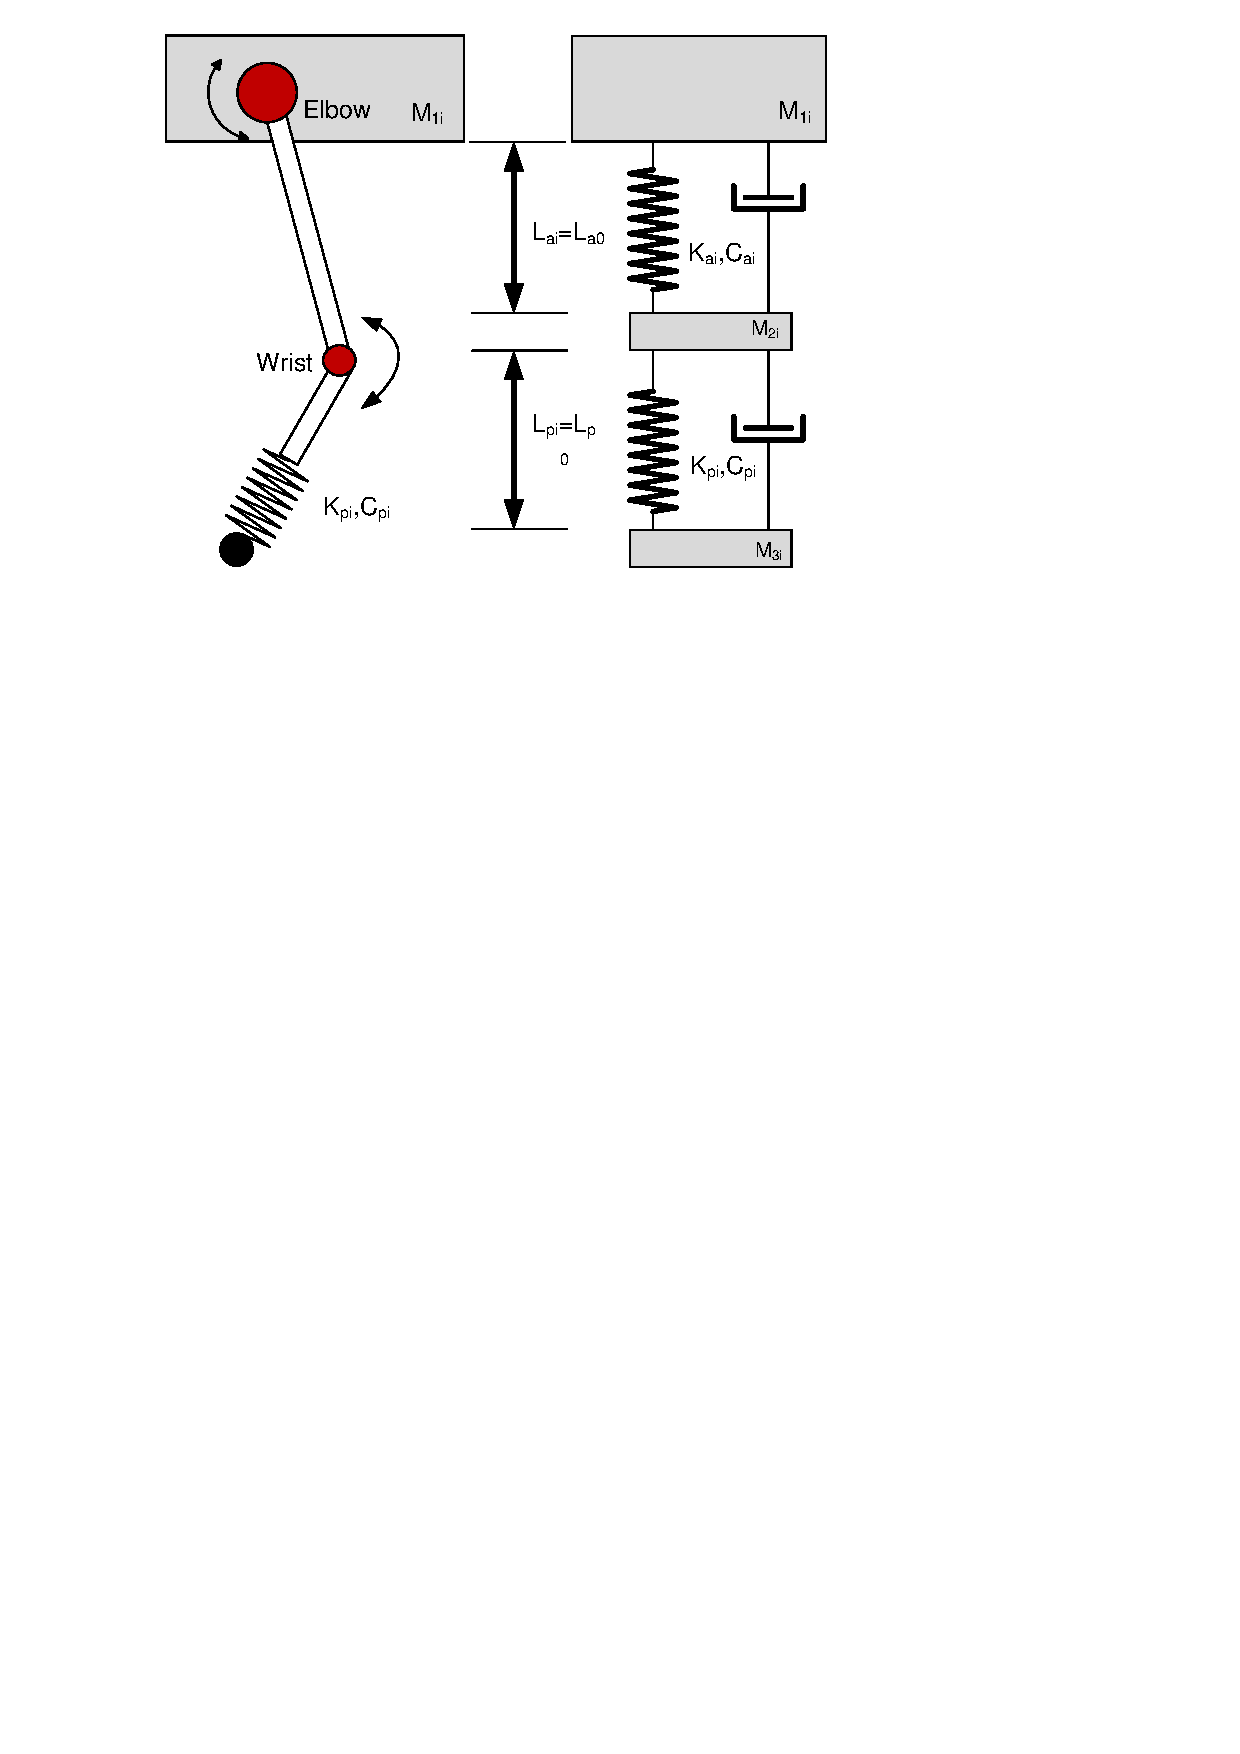
\includegraphics[width=80mm]{./pictures/Dynarobin_leg.pdf}
	\caption{Double spring-mass model of the leg}
	\label{fig:DynarobinLEG}
\end{figure}


%As it was previously explained, we propose modeling quadruped's legs as active springs. This can be achieved through adequate leg joint path planning, so that when the legs are in the contact with the ground, side forces and thrust forces are produced. 
Positioned symmetrically around the geometric center the legs exert forces and torques on the quadruped main body according to:

\begin{gather}\label{eq:Forces}
\vec{\textbf{F}_{tot}}=\sum_{i=1}^{4}(\vec{\textbf{T}_{i}}+\vec{\textbf{S}_{i}})\\
\vec{\boldsymbol{\tau}_{tot}}=\sum_{i=1}^{4}\vec{\boldsymbol{\rho} _i}\times(\vec{\textbf{T}_{i}}+\vec{\textbf{S}_{i}})
\end{gather}  
where $\vec{\textbf{T}_{i}}$ represents the $i$-th body part thrust force that causes vertical movement (i.e. hopping), $\vec{\textbf{S}_{i}}$ $i$-th cuboid side force that moves the quadruped in x direction, and $\vec{\boldsymbol{\rho}} _i$ denotes the $i$-th distance between the center mass and the origin of forces ($\vec{\boldsymbol{\rho}} _i=\vec{\textbf{r}} _CM+\vec{\textbf{r}} _i$). In reality, one would have the lateral component of the side force, but since this component is of the order of magnitude smaller then the sagittal component, it can be disregarded.

For a perfectly symmetric body the total torque (\ref{eq:Forces}) acting on the body is equal to zero, and the total force is the sum of all 4 active springs. For this, the necessary condition is that all four springs have exactly the same parameters (i.e. force magnitudes, distance from the geometric center, etc.), and thus exert the same forces. In reality, neither the springs are the same, nor can there be a perfectly symmetric body. We write the body torque equation for a non-symmetric body, with the center of mass displaced for $\vec{\Delta\textbf{r}_{CM}}$:

\begin{equation}\label{eq:Torques}
\vec{\boldsymbol{\tau}}_{tot}=\begin{bmatrix}
\Delta \textsc{y}_{CM} \:\bar{T} & -\left ( \Delta \textsc{x}_{CM} \:\bar{T} +\Delta \textsc{z}_{CM} \:\bar{S}\right ) & -\Delta \textsc{y}_{CM} \:\bar{S}
\end{bmatrix}^T
\end{equation}
where $\bar{T}$ and $\bar{S}$ represent the average thrust and side forces of each leg. The displacement of the center of mass is used to model the unbalanced body dynamics. In practice, the displacement vector  $\vec{\Delta\textbf{r}_{CM}}$ incorporates all possible imperfections: design asymmetry, leg differences, motor dynamics, unbalanced  forces and so on.

In order to achieve successful gallop locomotion which consists of a combined jump and forward movement, average forces $\bar{T}$ and $\bar{S}$ must exist. On the other hand, for a jumping part of the maneuver to remain stable, we need to counteract the undesired torque (\ref{eq:Torques}). Therefore, we propose, adding a tail to the quadruped in order to balance the robot and eliminate the undesired asymmetry. 

\subsection{Tail dynamics}
In order to devise a mathematical model of tail dynamics, we propose modeling the tail as an actuated kinematic chain manipulator attached to the robot body. Much like in aerial robots, when the robot is in the air \cite{Korpela2013ICRA,Orsag2012JINT}, the tail acts freely on its body. We aim to use the tail as a means to dynamically stabilize the hopping. First we build the kinematic model using Denavit-Hartenberg parameterization method, after that we devise a dynamic model of the tail using the recursive Newton-Euler algorithm.
\subsubsection{Complete kinematic and dynamic tail model}
kinematic chain of the tail is shown in Fig. \ref{fig:rmax}, and the kinematic parameters are shown in Table \ref{tab:DHParameters}. Kinematic chain consists of the body coordinate system, two tail revolute joints, one virtual prismatic joint in the tail (i.e. tail length parameter), and the tail center of mass coordinate system. As can be seen from Table \ref{tab:DHParameters}, the two revolute joints have no linear, only angular displacement from each other, therefore their masses and moments of inertia are all zero. The third prismatic joint represents the tail length and is modeled as a long stick with infinitesimal thickness. Normally, kinematic chains end with a tool at the tip of the last link, but here, the end effector is actually the tail center of mass, and thus it acts as the "tool" coordinate system.

\begin{table}
	\centering
		\begin{tabular}{ccccc}
		\hline
			& $\theta$ & $d$ & $a$ & $\alpha$ \\\hline
			\multicolumn{5}{c}{Body}\\\hline
			$B-0$ & $0$ & $d_B$ & $a_B$ & $0$\\\hline
			\multicolumn{5}{c}{Tail}\\\hline
			Joint 1 & $q_1$ & $0$ & $0$ & $-\frac{\pi}{2}$\\
			Joint 2 & $q_2$ & $0$ & $0$ & $\frac{\pi}{2}$\\
			Virtual joint& $0$ & $q_3$ & $0$ & $0$\\\hline
		\end{tabular}
	\caption{Denavit-Hartenberg Parameters}\label{tab:DHParameters}
\end{table}

The corresponding kinematic chain transformation matrix:
\begin{equation}\label{eq:T03}
\textbf{T}_0^3=\begin{bmatrix}
C_1 C_2 & -S_1 & C_1 S_2 & C_1 S_2 q_3 \\
C_2 S_1 & C_1 & S_1 S_2 & S_1 S_2 q_3 \\
-S_2 & 0 & C_2 & C_2 q_3 \\
 0 & 0 & 0 & 1
\end{bmatrix}
\end{equation}
with a standard abbreviation $Cos(q_1):=C_1$ $Sin(q_2):=S_2$ completes the Kinematic model of the tail. 

For this analysis we place the tail in the geometric center of the quadruped, $L_C$. Therefore, the distances between $L_0$ and $L_c$, $d_B$ and $a_B$ respectively, are both equal to zero. Using the recursive Newton-Euler method to build upon the kinematic model, we can write the complete dynamic model of the robot, which takes the following general form:

\begin{equation}\label{eq:NEGeneral}
\vec{\boldsymbol{\tau}}_B=\mathbf{D}\left ( \ddot{q_i},\vec{\boldsymbol{\alpha}}_B \right )+\mathbf{C}\left ( \dot{q_i},\vec{\boldsymbol{\omega}}_B \right )+\mathbf{H}\left ( {q_i} \right )
\end{equation}

The first term in \eqref{eq:NEGeneral}, $\mathbf{D}$ takes into account the tail joint accelerations $\ddot{q}_i$ and the body initial angular acceleration $\vec{\boldsymbol{\alpha}}_B$. Next are the Coriolis and centrifugal forces contained in $\mathbf{C}$, where the forces are produced from the coupling of joint velocities $\dot{q}_i$ and body angular speed $\vec{\boldsymbol{\omega}}_B$. The term $\mathbf{H}$ contains the gravity part of the equation. In a stand-still situation, when the robot is at rest and angular velocities and accelerations,  $\vec{\boldsymbol{\omega}}_B$ and  $\vec{\boldsymbol{\alpha}}_B$ are zero vectors, then the inertial acceleration, Coriolis and gravitational part of the equations take the following forms:
 
\begin{gather}\label{eq:DCH_matrix}
\small
\mathbf{D}\left ( \ddot{q_i},\vec{\boldsymbol{0}} \right )=\frac{m_T q_3^2}{24}\begin{bmatrix}
-3C_{q_1}S_{2q_2}\ddot{q_1} -8S_{q_1}\ddot{q_2}\\ -3S_{q_1}S_{2q_2}\ddot{q_1} +8C_{q_1}\ddot{q_2} \\ 8S_{q_2}\ddot{q_1}
\end{bmatrix} \\
\footnotesize
\mathbf{C}\left ( \dot{q_i},\vec{\boldsymbol{0}} \right )=\frac{m_T q_3^2}{24} \begin{bmatrix}
3S_{q_1}S_{22}{\dot{q_1}}^2-2C_{q_1}(5+3C_{22})\dot{q_1}\dot{q_2}\\ 
3C_{q_1}S_{22}{\dot{q_1}}^2-2S_{q_1}(5+3C_{22})\dot{q_1}\dot{q_2}\\ 
6S_{2q_2}\dot{q_1}\dot{q_2}
\end{bmatrix}\\
\small
\mathbf{H}\left ( {q_i} \right )=\frac{m_T q_3^2}{24} \begin{bmatrix}
-12S_1S_2g\\ 
12C_1S_2g\\ 
0
\end{bmatrix}
\normalsize
\end{gather}

\begin{figure}
	\centering
	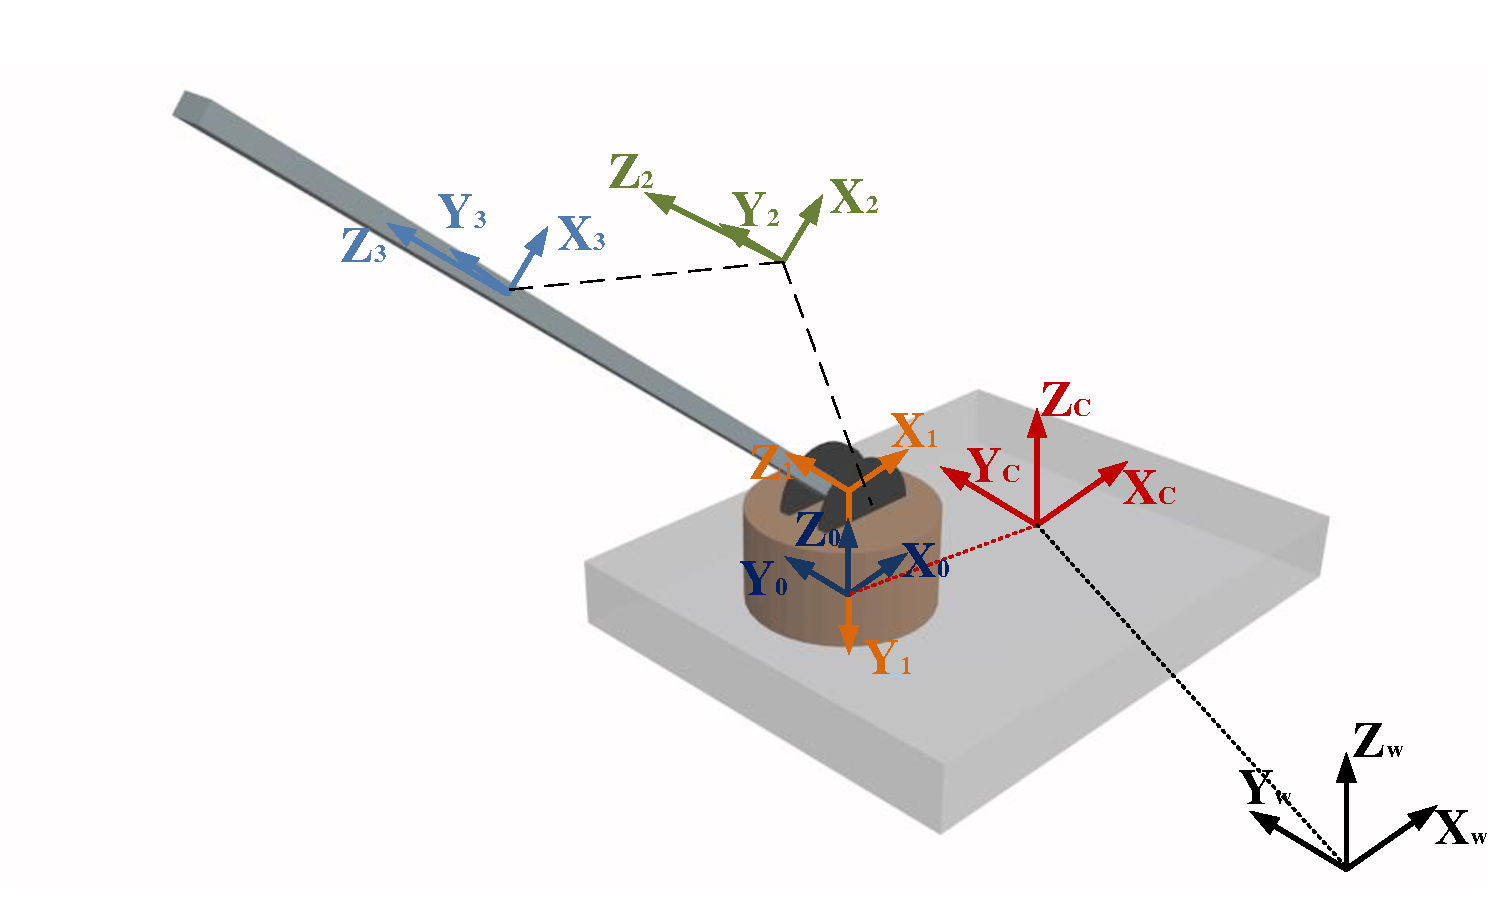
\includegraphics[width=85mm]{./pictures/RobinRepic.pdf}
	\caption{Robin Tail kinematic chain model}
	\label{fig:rmax}
\end{figure}

where $g=\left \| \vec{\mathbf{g}} \right \|$, the gravity acceleration and the additional abbreviations used are $Sin(q_i+q_j)=S_{ij}$. Equations \eqref{eq:DCH_matrix} show the full complexity of \eqref{eq:NEGeneral} even for a particular case when the quadruped body is at rest. The additional abbreviations used in these equations are $Sin(q_i+q_j)=S_{ij}$.Therefore it is clear, that an analytical solution to the problem of dynamic stabilization through tail motion is not a straight forward process. Instead, we propose using a tail to compensate the imperfections in quadruped construction. Positioning the tail at the right pose, it is possible to shift the balance of the robot and make it symmetric. 
\subsubsection{Tail inertia tensor}
in Fig. \ref{fig:rmoment}, a tail with its ${L_T}$ coordinate system, placed in its center of mass is depicted. Upon introducing the tail as a new body part in the quadruped construction, the overall center of mass will change accordingly:
\begin{equation}\label{eq:CMrobotAndTail}
\vec{\textbf{r}_{CM}}=\frac{\sum_{i=1}^{4}m_i\vec{\textbf{r}}_i+m_T\vec{\textbf{p}}_T}{\sum_{i=1}^{4}m_i+m_T}= \frac{\Delta\vec{\textbf{r}_{CMB}}+\mu\cdot\vec{\textbf{r}_{CMT}}}{1+\mu}
\end{equation}


In the previous equation we introduced the mass ratio $\mu=\frac{m_T}{\sum_{i=1}^{4}m_i}$ and $\Delta\vec{\textbf{r}_{CM}}$ as the center of mass of the robot without the tail, from equation (\ref{eq:CMrobot}). If we are to keep the center of mass in the construction center of the robot (i.e. $\vec{\textbf{r}_{CM}}=0$), then the following condition has to be met:
\begin{equation}\label{eq:CMzeroing}
\begin{bmatrix}
\Delta \textsc{x}_{cm}\\ 
\Delta \textsc{y}_{cm}\\ 
\Delta \textsc{z}_{cm}
\end{bmatrix}+
\frac{\mu q_3}{2}\begin{bmatrix}
C_1S_2\\ 
S_1S_2\\ 
C_2
\end{bmatrix}=0
\end{equation}
that is to say, that the numerator in (\ref{eq:CMrobotAndTail}) has to be zero. Given that in (\ref{eq:CMzeroing}) there exist only two variables, $q_1$ and $q_2$ respectively, one can eliminate only two components of the center of mass displacement vector $\Delta \vec{\textbf{r}_{CM}}$. Under a reasonable assumption that $\bar{T}\gg \bar{S}$, it follows from the applied torque equation (\ref{eq:Torques}) that for a stable jump one needs to successfully eliminate $x$ and $y$ components of the center of mass displacement vector. This hypothesis is reasonable because in most cases the forward motion is slow compared to vertical jumping, and additionally in z direction one needs to overcome the gravity acceleration $g$. Combining these two assumptions makes the $\bar{T}$ by the order of magnitude larger than $\bar{S}$.

From a strict mathematical point of view, the necessary condition for (\ref{eq:CMzeroing}) to have a solution is:
\begin{equation}\label{eq:CMcondition}
\frac{\mu q_3}{2}\geq \textup{MAX}\left \{ \left | \Delta \textsc{x}_{CM} \right |, \left | \Delta \textsc{y}_{CM} \right |,\left | \Delta \textsc{z}_{CM} \right |\right \}
\end{equation}
When the condtion (\ref{eq:CMcondition}) is met, the analytical solution to equation (\ref{eq:CMzeroing}) can easily be derived:
\begin{gather}\label{eq:CMsolution1}
q_1=atan2\left({\Delta \textsc{y}_{CM}},\, {\Delta \textsc{x}_{CM}}\right)\\
q_2=asin\left(\frac{2\sqrt{{\Delta \textsc{x}_{CM}}^2+{\Delta \textsc{y}_{CM}}^2}}{\mu q_3} \right)\label{eq:CMsolution2}
\end{gather}
Moving the tail joints $q_1$ and $q_2$ to the values calculated with \eqref{eq:CMsolution1} and \eqref{eq:CMsolution2} respectively, balances the quadruped. On the other hand, repositioning the tail changes the overall inertia tensor. This change in the overall inertia can be calculated using the Parallel axis theorem and basic rotation matrices. We start by writing the tail inertia tensor, which, due to the approximation that the tail is infinitesimally thin, can be simplified. Written in $L_T$ frame, the tail moment of inertia is:
\begin{equation}\label{eq:JT_LT}
\textbf{J}_T=\textbf{J}_3=\frac{{q_3}^2 m_T}{12}\left(
\begin{array}{ccc}
 1 & 0 & 0 \\
 0 & 1 & 0 \\
 0 & 0 & 0
\end{array}
\right)
\end{equation}
However, in order to write \eqref{eq:JT_LT} in the body coordinate system $L_B$ it needs to be rotated first. After that, the Parallel axis theorem is applied, yielding the equation for the tensor of inertia $J_T$ of the tail. 
\begin{equation}
\begin{aligned}
\scriptsize
{\textbf{J}_T}^*={\textbf{R}_0^3}^T\textbf{J}_T\textbf{R}_0^3+\\+m_T\begin{bmatrix}
{cm_y^T}^2 +{cm_z^T}^2& {cm_x^T}{cm_y^T}& {cm_x^T}{cm_z^T} \\ 
-{cm_x^T}{cm_y^T} & {cm_x^T}^2+{cm_z^T}^2 & {cm_y^T}{cm_z^T}\\ 
-{cm_x^T}{cm_z^T} & -{cm_y^T}{cm_z^T} & {cm_x^T}^2+{cm_y^T}^2
\end{bmatrix}
\normalsize
\end{aligned}
\end{equation}
with $\textbf{R}_0^3$ as a rotation submatrix in \eqref{eq:T03}. Finally, the total moment of inertia is then a sum of the body moment of inertia $\textbf{J}_B$ and the tail moment of inertia $\textbf{J}_T^*$, both written in the body coordinate system.
\begin{equation*}
\textbf{J}_{tot}=\textbf{J}_B+\textbf{J}_T^*
\end{equation*}


%%%%%%%%%%%%%%%%%%%%%%%%%%%%%%%%%%%%%%%

%%%%%%%%%%%%%%%%%%%%%%%%%%%%%%%%%%%%%%%
% Mathematical model
\section{Iterative center of mass displacement compensation algorithm}\label{sec:Algorithm}
In reality, the distribution of the center of mass within the body is not known, and therefore, an analytic solution provided with (\ref{eq:CMsolution2}) is impossible to calculate, thus an iterative method, based on repetitive hopping response is proposed. When a quadruped is continuosly jumping, its contact with the ground is infitesimally short, and consequently, reaction forces and torques can be approximated with the Dirac function $\delta (s)$. During the jump, the body behaves according to the Euler body dynamics function (\ref{eq:EulerBody}). Taking account the infitessimally short time the body has to accelerate (i.e. the rotation speeds are small, and their product is event smaller) the cross coupling term $\vec{\omega}\times J_B\vec{\omega}$ can be neglected and, consequently, the rotation speed vector can be approximated with (\ref{eq:RotSpeedAprox}).
\begin{figure}
	\centering
	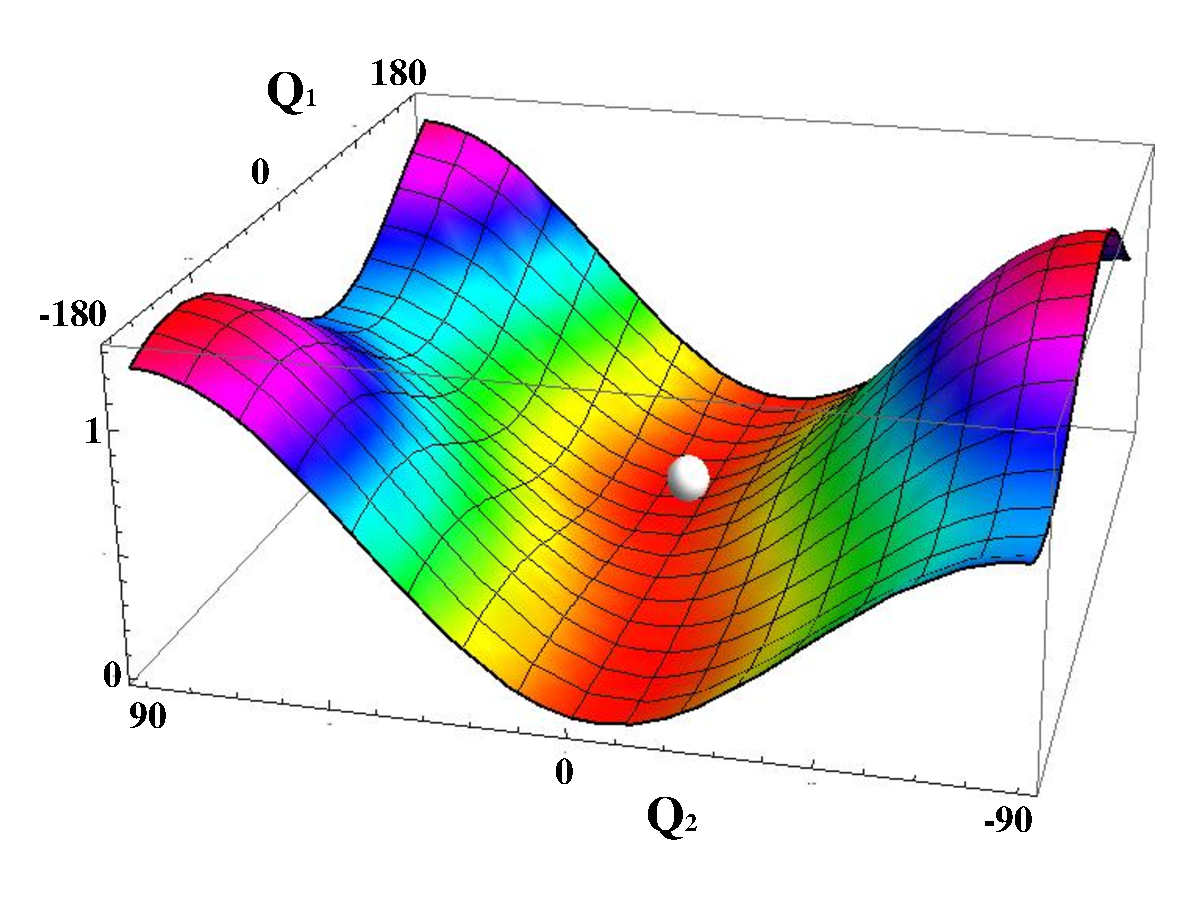
\includegraphics[width=85mm]{./pictures/RobinRepicCM.pdf}
	\caption{Center of mass displacement}
	\label{fig:CM3Dfunction}
\end{figure}

\begin{equation}\label{eq:EulerBody}
\tau_{tot}=J_B\vec{\dot{\omega}}+\vec{\omega}\times J_B\vec{\omega}
\end{equation}

\begin{equation}\label{eq:RotSpeedAprox}
\vec{\omega}\approx \frac{1}{s}{J_B}^{-1}\begin{bmatrix}
\Delta \textsc{cm}_y & -\Delta \textsc{cm}_x & 0
\end{bmatrix}^T\bar{T}\delta(s)
\end{equation}

Calculating the absolute value of vector (\ref{eq:RotSpeedAprox}) it is easy to show that the size of the rotation speed vector is proportional to the displacement of center of mass \eqref{eq:WpropCM}. In other words, centering the robot and minimizing the displacement of the center of mass eliminates the generation of unwanted rotations. 

\begin{equation}\label{eq:WpropCM}
\left \| \vec{\omega} \right \|\sim \sqrt{{\Delta \textsc{cm}_x}^2+{\Delta \textsc{cm}_y}^2}
\end{equation}


In order to iteratively calculate the angles $q1$ and $q2$, angular velocity vector is recorded during beginning of hopping acceleration phase. The initial actuated spring value $L_{i0}$ is changed by value $\delta L$:

\begin{equation}
\tiny
L_{i1}=L_{i0}+\delta L
\normalsize
\end{equation}  

This phase is completed ($t_{JC}$) until one of the leg/spring reaches desired length $L_{i1}$. The leg which carries a minimum mass will achieve the fastest acceleration and the algorithm task is to navigate tail towards this leg. At the end of acceleration phase the body rotates at an angular velocity $\vec{\omega}(t_{JC})$. By using the cross product of projection vector $\vec{\omega_{xy}}$ in $XY$ plane and body $\vec{Zb}$, the tail direction vector $\vec{\omega_{TD}}$ is calculated (see Fig.\ref{fig:imassCom}). The tail motion control algorithm navigates tail in $\vec{\omega_{TD}}$ direction by using the simple P($K_o$) regulation. The algorithm finishes when $\left \| \vec{\omega}(t_{JC}) \right \|\ $ is smaller than predefined limit value $\omega_{max}$.  For example, the mass distribution in Fig.\ref{fig:imassCom} is equally distributed except for $MASS_2$  which is lighter then others. As expected, the iterative algorithm will navigate tail towards that mass.



\begin{algorithm}
\caption{Minimize $\left \| \vec{\omega} \right \|\sim \sqrt{{\Delta \textsc{cm}_x}^2+{\Delta \textsc{cm}_y}^2}$}
\begin{algorithmic} 
\STATE $y \leftarrow 1$
\REPEAT
\STATE $Q_1 \leftarrow$ initial value
\STATE $Q_2 \leftarrow$ initial value
\STATE JUMP

\REPEAT
\STATE recording $\vec{\omega}(t)$
\UNTIL JUMP COMPLETE
\STATE $\vec{\omega_{TD}} = \vec{\omega_{xy}}(t_{JC}) \times \vec{Zb}$
\STATE Move tail in $\vec{\omega_{TD}}$ direction - gain $K_o$
\UNTIL{$\left \| \vec{\omega}(t_{JC}) \right \|\ < \omega_{max}$}
\end{algorithmic}
\end{algorithm}


\begin{figure}
	\centering
	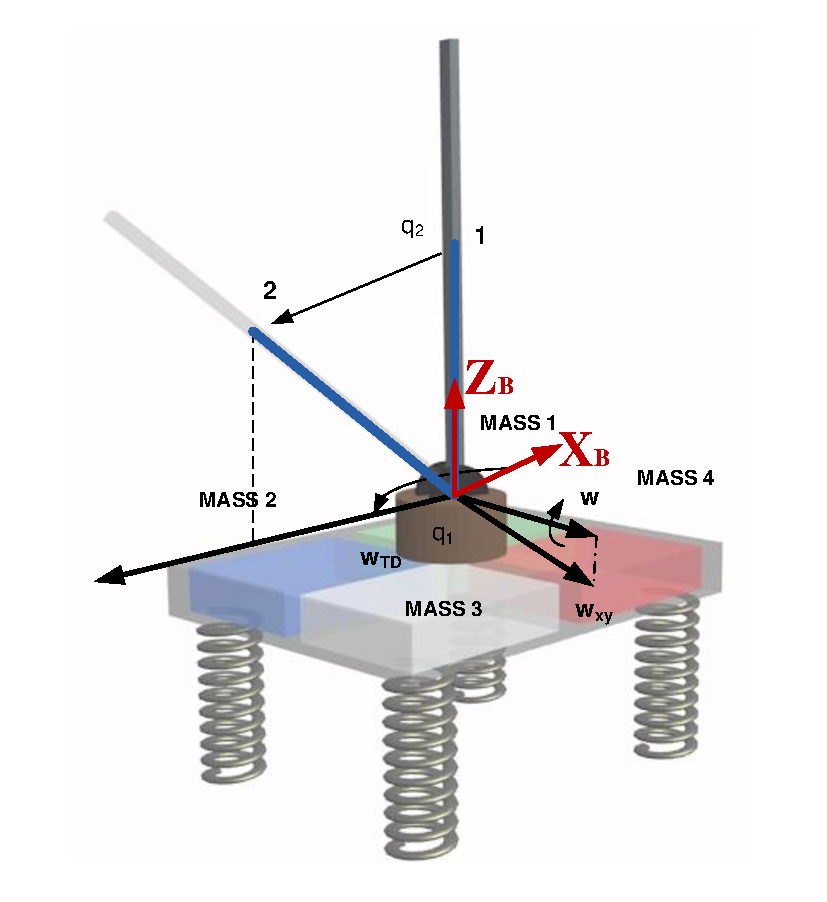
\includegraphics[width=85mm]{./pictures/IterativeAlgorithm.pdf}
	\caption{Iterative mass displacement compensation}
	\label{fig:imassCom}
\end{figure}

%%%%%%%%%%%%%%%%%%%%%%%%%%%%%%%%%%%%%%%

%%%%%%%%%%%%%%%%%%%%%%%%%%%%%%%%%%%%%%%
% Simulations
\section{Simulations}\label{sec:simulation}

The ODE (Open Dynamics Engine) library \cite{ode:2008} is used to test the iterative mass displacement compensation algorithm presented in the previous section. The initial position of the hopping quadruped robot is shown in Fig \ref{fig:ODESimulations}a. Each leg is composed of two spring-damper joints, the first, passive, connects the red and green cylinder together; and the second, active one, connects the green cylinder with the robot body. The body consists of 4 composite masses indexed as 1 (white), 2 (red), 3 (green) and 4 (blue). All the parameters of the  robot simulation are shown in Table \ref{tab:RobotDimensions}.

\begin{table}[!t]
\centering
\begin{tabular}{|c|c|}
	\hline
	$Body\: size$ &  $[0.30\: 0.15\: 0.01]m$ \\
	\hline
	$Lower\:leg\:size$ &  $0.05m$ \\
	\hline
	$Upper\:leg\:size$ &  $0.05m$ \\
	\hline
	$Leg\:radius$ &  $0.01m$ \\
	\hline
	$Total\:leg\:mass$ &  $0.15kg$ \\
	\hline
	$Passive\:spring\:k/c$ &  $2000N/m, 50Ns/m$ \\
	\hline
	$Active\:spring\:k/c$ &  $10000N/m, 30Ns/m$ \\
	\hline
	$Tail\:length$ &  $0.1m$ \\
	\hline
	$Tail\:radius$ &  $0.005m$ \\
	\hline
\end{tabular}
\caption{Robot simulation parameters}\label{tab:RobotDimensions}
\end{table}



Active springs generate forces periodically with the period interval $Td=1s$ which accelerate the body and produce rotational vector which is recorded during the acceleration phase. The applied spring force is minimal, but sufficient enough to produce measurable angular speed and to keep the time needed to calm the body oscillations down to a minimum. The acceleration phase lasts for about 200ms after which the body calms in the next 800ms. The initial tail angles are $q_1=0$ and $q_2=0$ as illustrated in Fig. \ref{fig:ODESimulations}a.

\begin{table}[!t]
	\centering
\begin{tabular}{|c|c|c|c|c|}
	\hline
$Test$ &  $Mass[kg]$ & $q$  & $\left \| \vec{\boldsymbol{\omega}} \right \|$ & $K_0$\\
	\hline
1   & $[0\: 0\: 1\: 1]$ & $[89.99\: 32.86]$ & 0.0026 & 0.3\\
2   & $[1\: 1\: 0\: 0]$ & $[-89.99\: 32.20]$ & 0.0038 & 0.3\\
3   & $[1\: 1\: 1\: 0]$ & $[-25.43\: 29.15]$ &  0.003 & 0.3\\
4   & $[1\: 1\: 1\: 0]$ & $[-23.26\: 29.20]$ &  0.003 & 0.6\\
\hline
\end{tabular}
\caption{Testing parameters}\label{tab:Simulations}
\end{table}



\begin{figure}[!t]
	\centering
	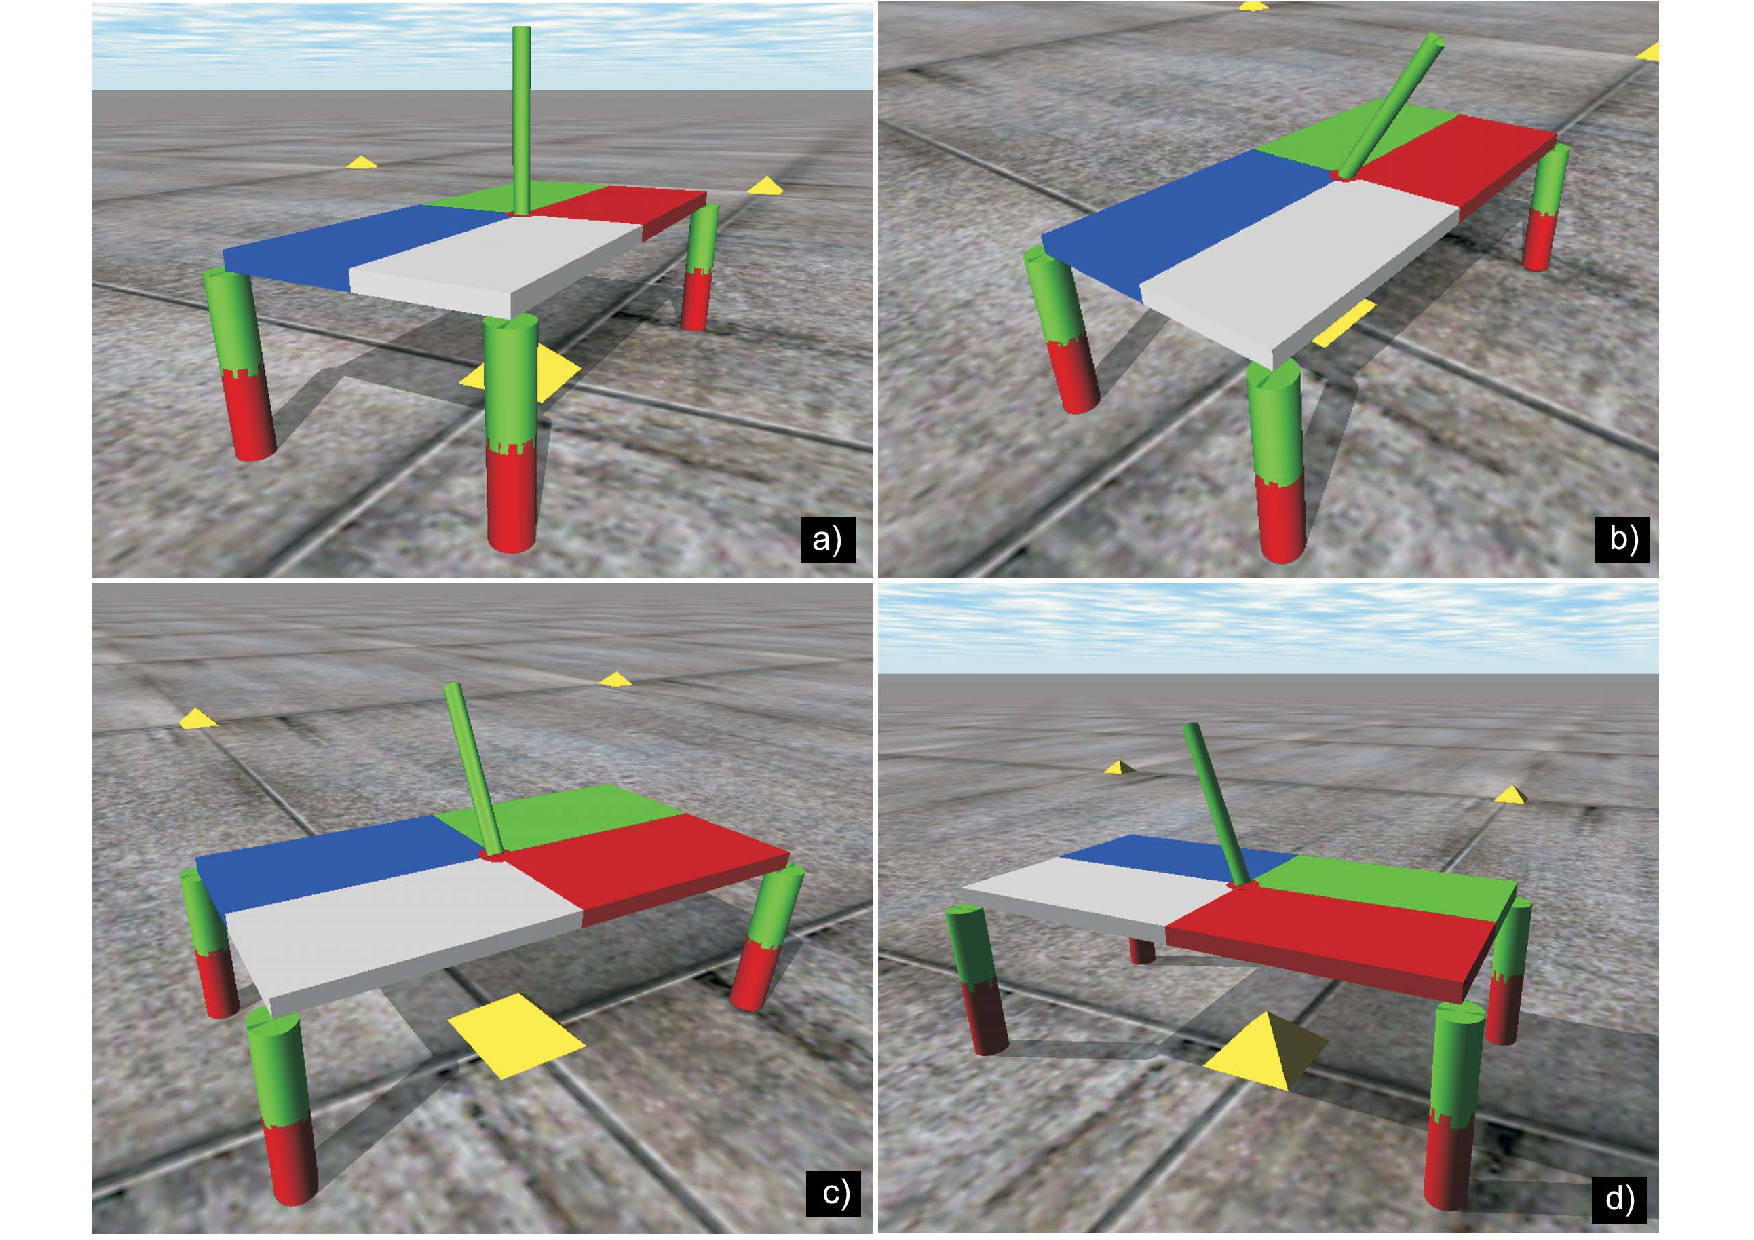
\includegraphics[width=80mm]{./pictures/ODE_simulations.pdf}
	\caption{ODE simulations. a) Initial position b) Test 1. c) Test 2. d) Test 3.}
	\label{fig:ODESimulations}
\end{figure}

A series of four experiments has been conducted by varying the initial mass distribution of the robot, as shown in Table \ref{tab:Simulations}. The first column represents body mass redistribution vector, while the second and the third are the final results of tail angles and angular velocity values, respectively. The simulation results are presented in Fig. \ref{fig:ODE graph}. 

Test 1: For negligibly small masses of white and red cuboids, the algorithm consequently tilts the tail in the direction $q1=90^{\circ}$. The tail reaches the desired position in 7-10 seconds and the final inclination is $q2=32.86^{\circ}$(Fig. \ref{fig:ODESimulations}b). The angular velocity value $\left \| \vec{\boldsymbol{\omega}} \right \|$ falls from $0.14$ to final $0.0025$.

Test 2: When the green and blue cuboid masses are negligible, the algorithm tilts the tail in the direction $q1=-90^{\circ}$. The final tail inclination is $q2=32.20^{\circ}$(Fig. \ref{fig:ODESimulations}c). The angular velocity value $\left \| \vec{\boldsymbol{\omega}} \right \|$ goes from $0.14$ to final $0.0038$. 

\begin{table}[!t]
	\centering
\begin{tabular}{|c|c|c|c|}
	\hline
$Interation$ & $q_1$ & $q_1$  & $\left \| \vec{\boldsymbol{\omega}} \right \|$\\
	\hline
1 & -53.71 & 10.19 & 0.060\\
5 & -36.89 & 21.75 & 0.012\\
10 & -32.44 & 27.03 &  0.005\\
15 & -29.09 & 28.81 & 0.004\\
20 & -25.43 & 29.15 &  0.003\\
\hline
\end{tabular}
\caption{Test 3. results}\label{tab:Simulations2}
\end{table}

Test 3: When only the blue cuboid mass is negligible, the algorithm tilts the tail in the direction $q1=-25.43^{\circ}$. The final tail inclination is $q2=29.15^{\circ}$(Fig. \ref{fig:ODESimulations}d). The algorithm requires a longer time to minimize $\left \| \vec{\boldsymbol{\omega}} \right \|$ to final $0.0025$ (see Table \ref{tab:Simulations2}).



Test 4: This experiment was conducted with the same initial parameters as in Test 3, except this time the higher gain $K_0$ was used. The desired position is reached faster as expected. The subsequent increase has shown to cause small oscillations in the result. By comparing Fig. 5, it is interesting to notice how joint angle $q_1$ takes more time to achieve the desired equilibrium. This is obvious, since according to Fig 5, once the algorithm reaches the saddle of equation (22), the slope in $q_1$ direction is very small.

A video showing the simulation results in the ODE environment is available at \cite{IROS2013Movie}.


\begin{figure*}[!t]
	\centering
	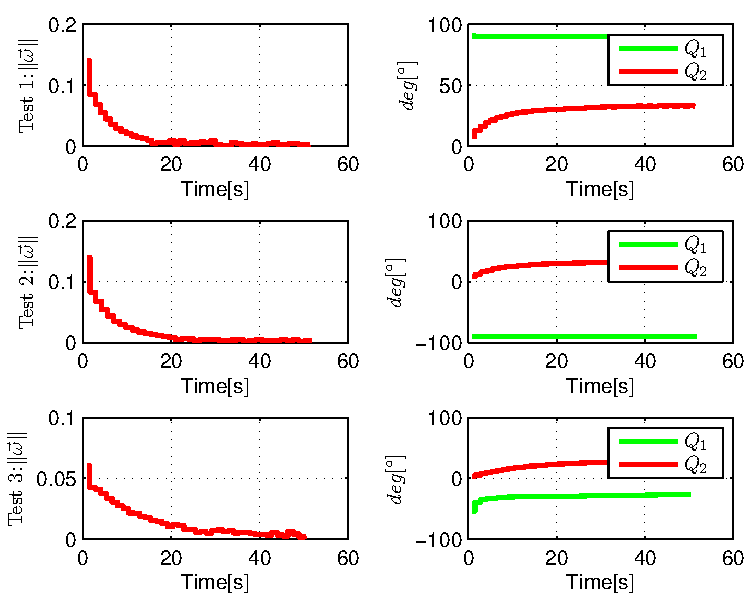
\includegraphics[width=111mm]{./pictures/ODE_graph.pdf}
	\caption{ODE simulations, Test 1-4.}
	\label{fig:ODE graph}
\end{figure*}





%%%%%%%%%%%%%%%%%%%%%%%%%%%%%%%%%%%%%%%

%%%%%%%%%%%%%%%%%%%%%%%%%%%%%%%%%%%%%%%
% Simulations
\section{Conclusion}\label{sec:conclusion}
 
The tail presented in the paper is used as a counterweight, capable of shifting its center of mass so as to balance the body of the robot. To that end, a recursive algorithm that moves the tail in order to balance the robot is proposed. In order to simplify the complexity of the analysis, quadruped's main body is modeled as a system of four, equally displaced cuboid shaped bodies. Varying the mass of each cuboid separately, it is possible to model the imperfections in the robot design. Impedance control implemented in robot leg joints makes it possible to model the complete leg behavior as a spring-mass system.   

Iterative center of mass displacement algorithm is introduced with the purpose of overcoming imperfections of the robot. The algorithm iteratively navigates the tail towards the optimal pose where its center of mass counteracts the shift in the body center. This minimizes the overall center of mass displacement; consequently the generated rotations during hopping become negligible. Four tests are conducted, that show how that algorithm can compensate unwanted rotations after minimum of 7 to 10 consecutive jumps.

Future work includes testing this algorithm on a real robot implementation so as to achieve a completely symmetric construction. Furthermore, dynamic stabilization based on the conservation of momentum should be implemented. Using these two methods should yield a stable quadruped dyanarobin galloping motion.



%%%%%%%%%%%%%%%%%%%%%%%%%%%%%%%%%%%%%%%

%%%%%%%%%%%%%%%%%%%%%%%%%%%%%%%%%%%%%%%%%%%%%%%%%%%%%%%%%%%%%%%%%%%%%%%%%%%%%%%%

%\addtolength{\textheight}{-4cm}   % This command serves to balance the column lengths
                                  % on the last page of the document manually. It shortens
                                  % the textheight of the last page by a suitable amount.
                                  % This command does not take effect until the next page
                                  % so it should come on the page before the last. Make
                                  % sure that you do not shorten the textheight too much.

%%%%%%%%%%%%%%%%%%%%%%%%%%%%%%%%%%%%%%%%%%%%%%%%%%%%%%%%%%%%%%%%%%%%%%%%%%%%%%%%

\bibliographystyle{bibliography/IEEEtran}
\bibliography{bibliography/IEEEabrv,bibliography/bibliography}

\end{document}
